%=================================================================
\section{Introduction}\label{sec-intro}


In this competition you are predicting the values of air pollution measurements over time, 
based on basic weather information (temperature and humidity) and the input values of 5 sensors.
The three target values to you to predict are:
\begin{itemize}
	\item target-carbon-monoxide
	\item target-benzene
	\item target-nitrogen-oxides
\end{itemize}


\section{Data Description} \label{sec-preliminaries}
Before model training, data needs to be analyzed to determine the required features. Here is the statistics of training data and test data:
	
\begin{table}[H]  \centering
	\caption{Train Data Description}
	\label{tbl:Train Data Description}
		\begin{tabular}{c| c }
		\toprule
		%\centering
		Elements & \texttt{Number}  \\
		\midrule
		$date time$
		&  {$7111$} \\
		$deg C$
		&  {$408$} \\
		$relative-humidity$
		&  {$762$}  \\
		$absolute-humidity$
		&  {$5451$}  \\
		$sensor 1$
		&  {$3882$} \\
		$sensor 2$
		&  {$3882$} \\
		$sensor 3$
		&  {$3882$} \\
		$sensor 4$
		&  {$3882$} \\
		$sensor 5$
		&  {$3882$} \\
		$target-carbon-monoxide$
		&  {$95$} \\
		$target-benzene$
		&  {$405$} \\
		$target-nitrogen-oxides$
		&  {$3268$} \\
		\bottomrule
	\end{tabular}
\end{table}

\begin{table}[H]  \centering
	\caption{Test Data Description}
	\label{tbl:Test Data Description}
	\begin{tabular}{c| c }
		\toprule
		%\centering
		Elements & \texttt{Number}  \\
		\midrule
		$date time$
		&  {$2247$} \\
		$deg C$
		&  {$280$} \\
		$relative-humidity$
		&  {$653$}  \\
		$absolute-humidity$
		&  {$1915$}  \\
		$sensor 1$
		&  {$1758$} \\
		$sensor 2$
		&  {$1816$} \\
		$sensor 3$
		&  {$1833$} \\
		$sensor 4$
		&  {$1877$} \\
		$sensor 5$
		&  {$2017$} \\
		\bottomrule
	\end{tabular}
\end{table}

In order to understand the change trend of data, the data is visualized and analyzed based on the visualization results.

\begin{figure}[H]
	\centering
	\selectcolormodel{rgb}
	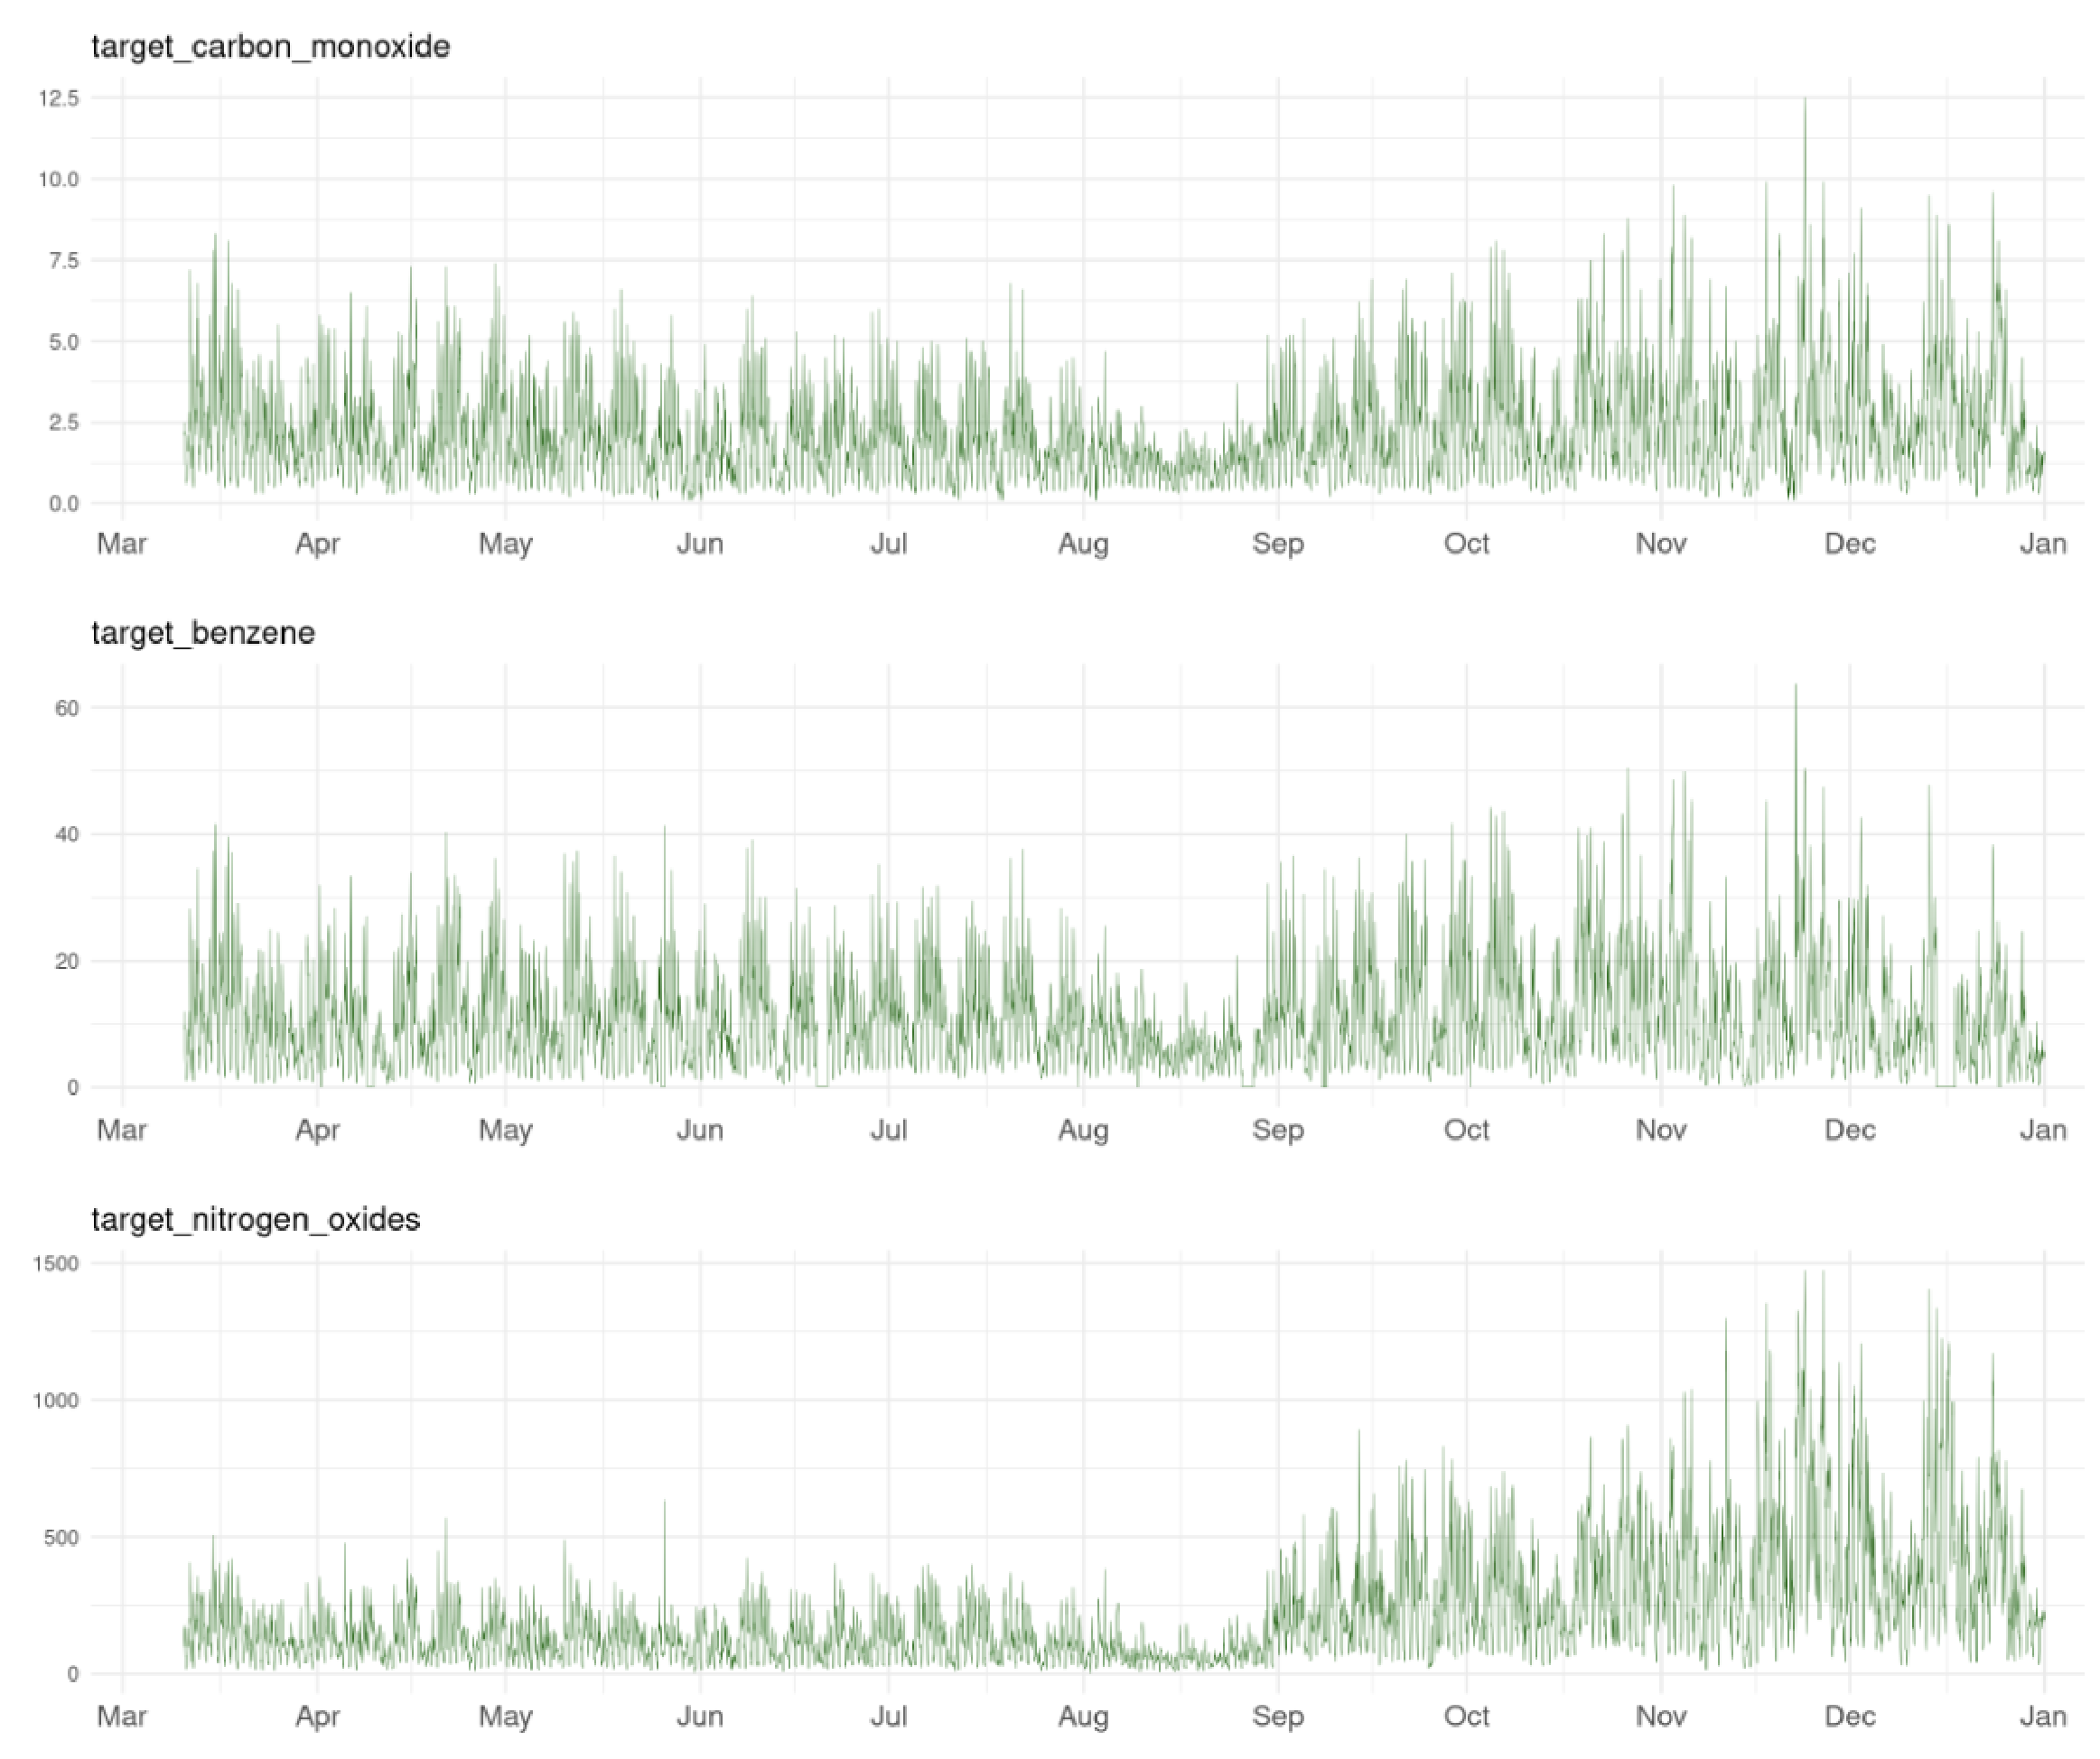
\includegraphics[scale=0.3]{figures//p1.eps}\\
	\caption{Target Overall Situation}\label{fig:Target Overall Situation}
\end{figure}
It can be seen from the figure1 that the values of the three target pollutants in August each year will be lower, 
gradually rising from September, and significantly higher than the level before August, 
so it is necessary to take the month as a feature of the model. 

\begin{figure}[H]
	\centering
	\selectcolormodel{rgb}
	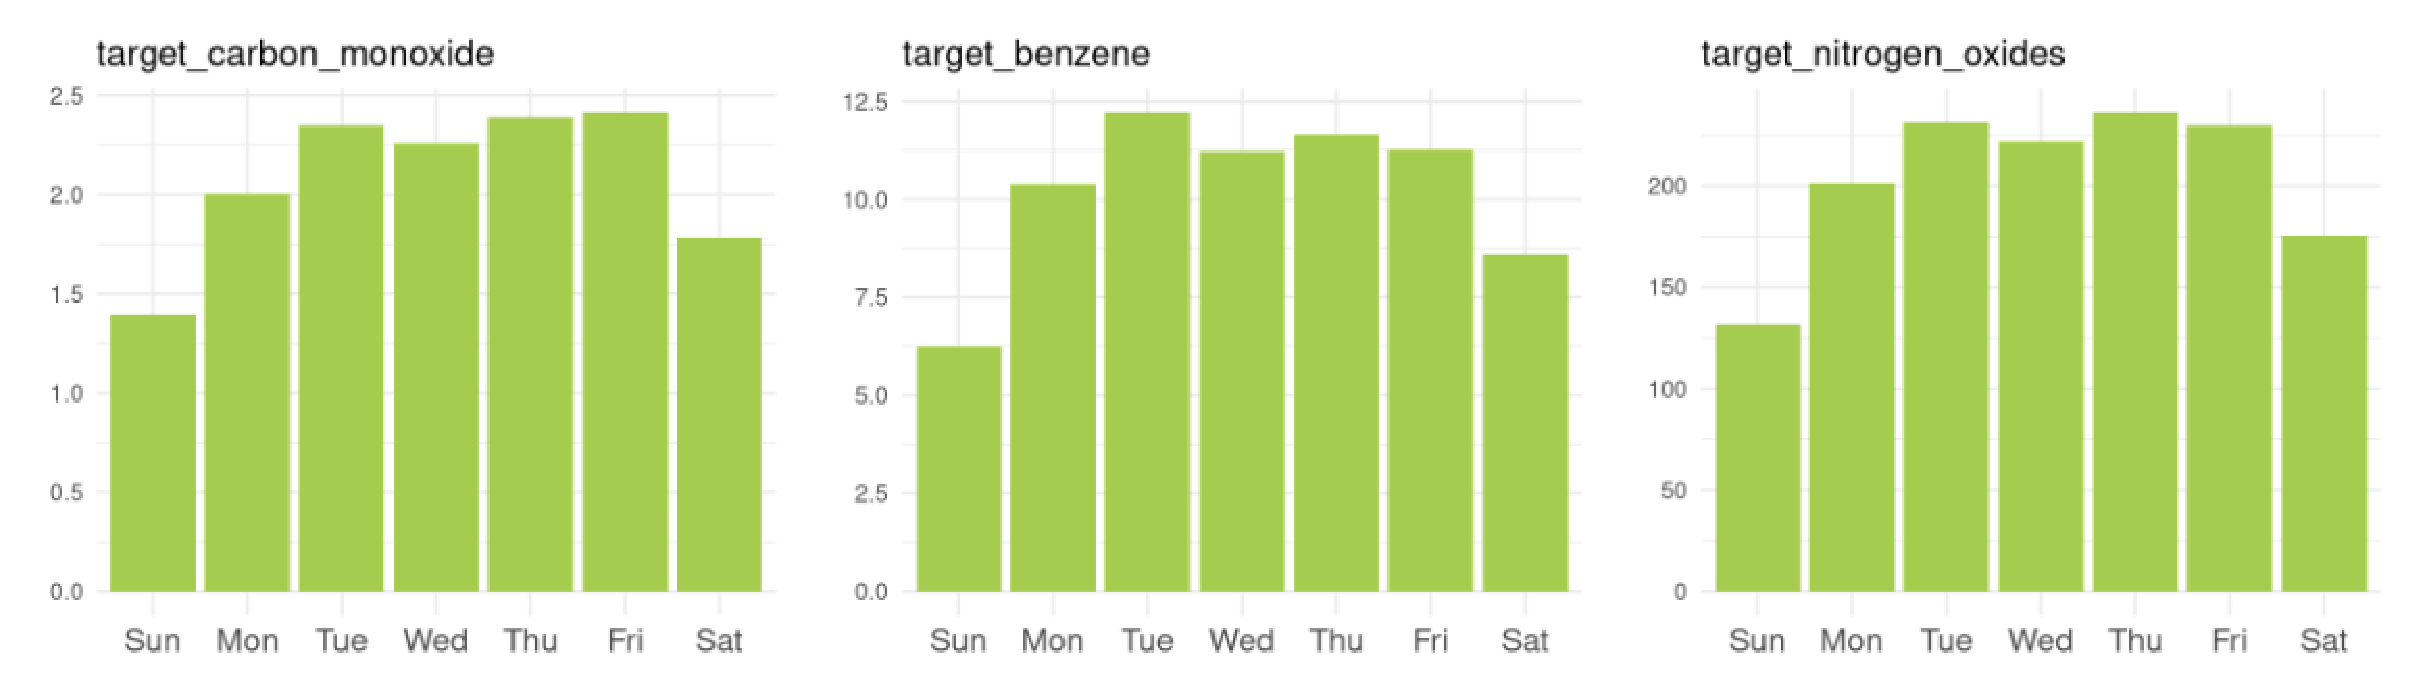
\includegraphics[scale=0.3]{figures//p9.eps}\\
	\caption{Target Weekly Situation}\label{fig:Target Weekly Situation}
\end{figure}
It can be seen from the figure2 that the content level of each pollutant at the weekend of each week will decrease significantly, so it is necessary to take whether this day is a weekend as a feature of the model.

\begin{figure}[H]
	\centering
	\selectcolormodel{rgb}
	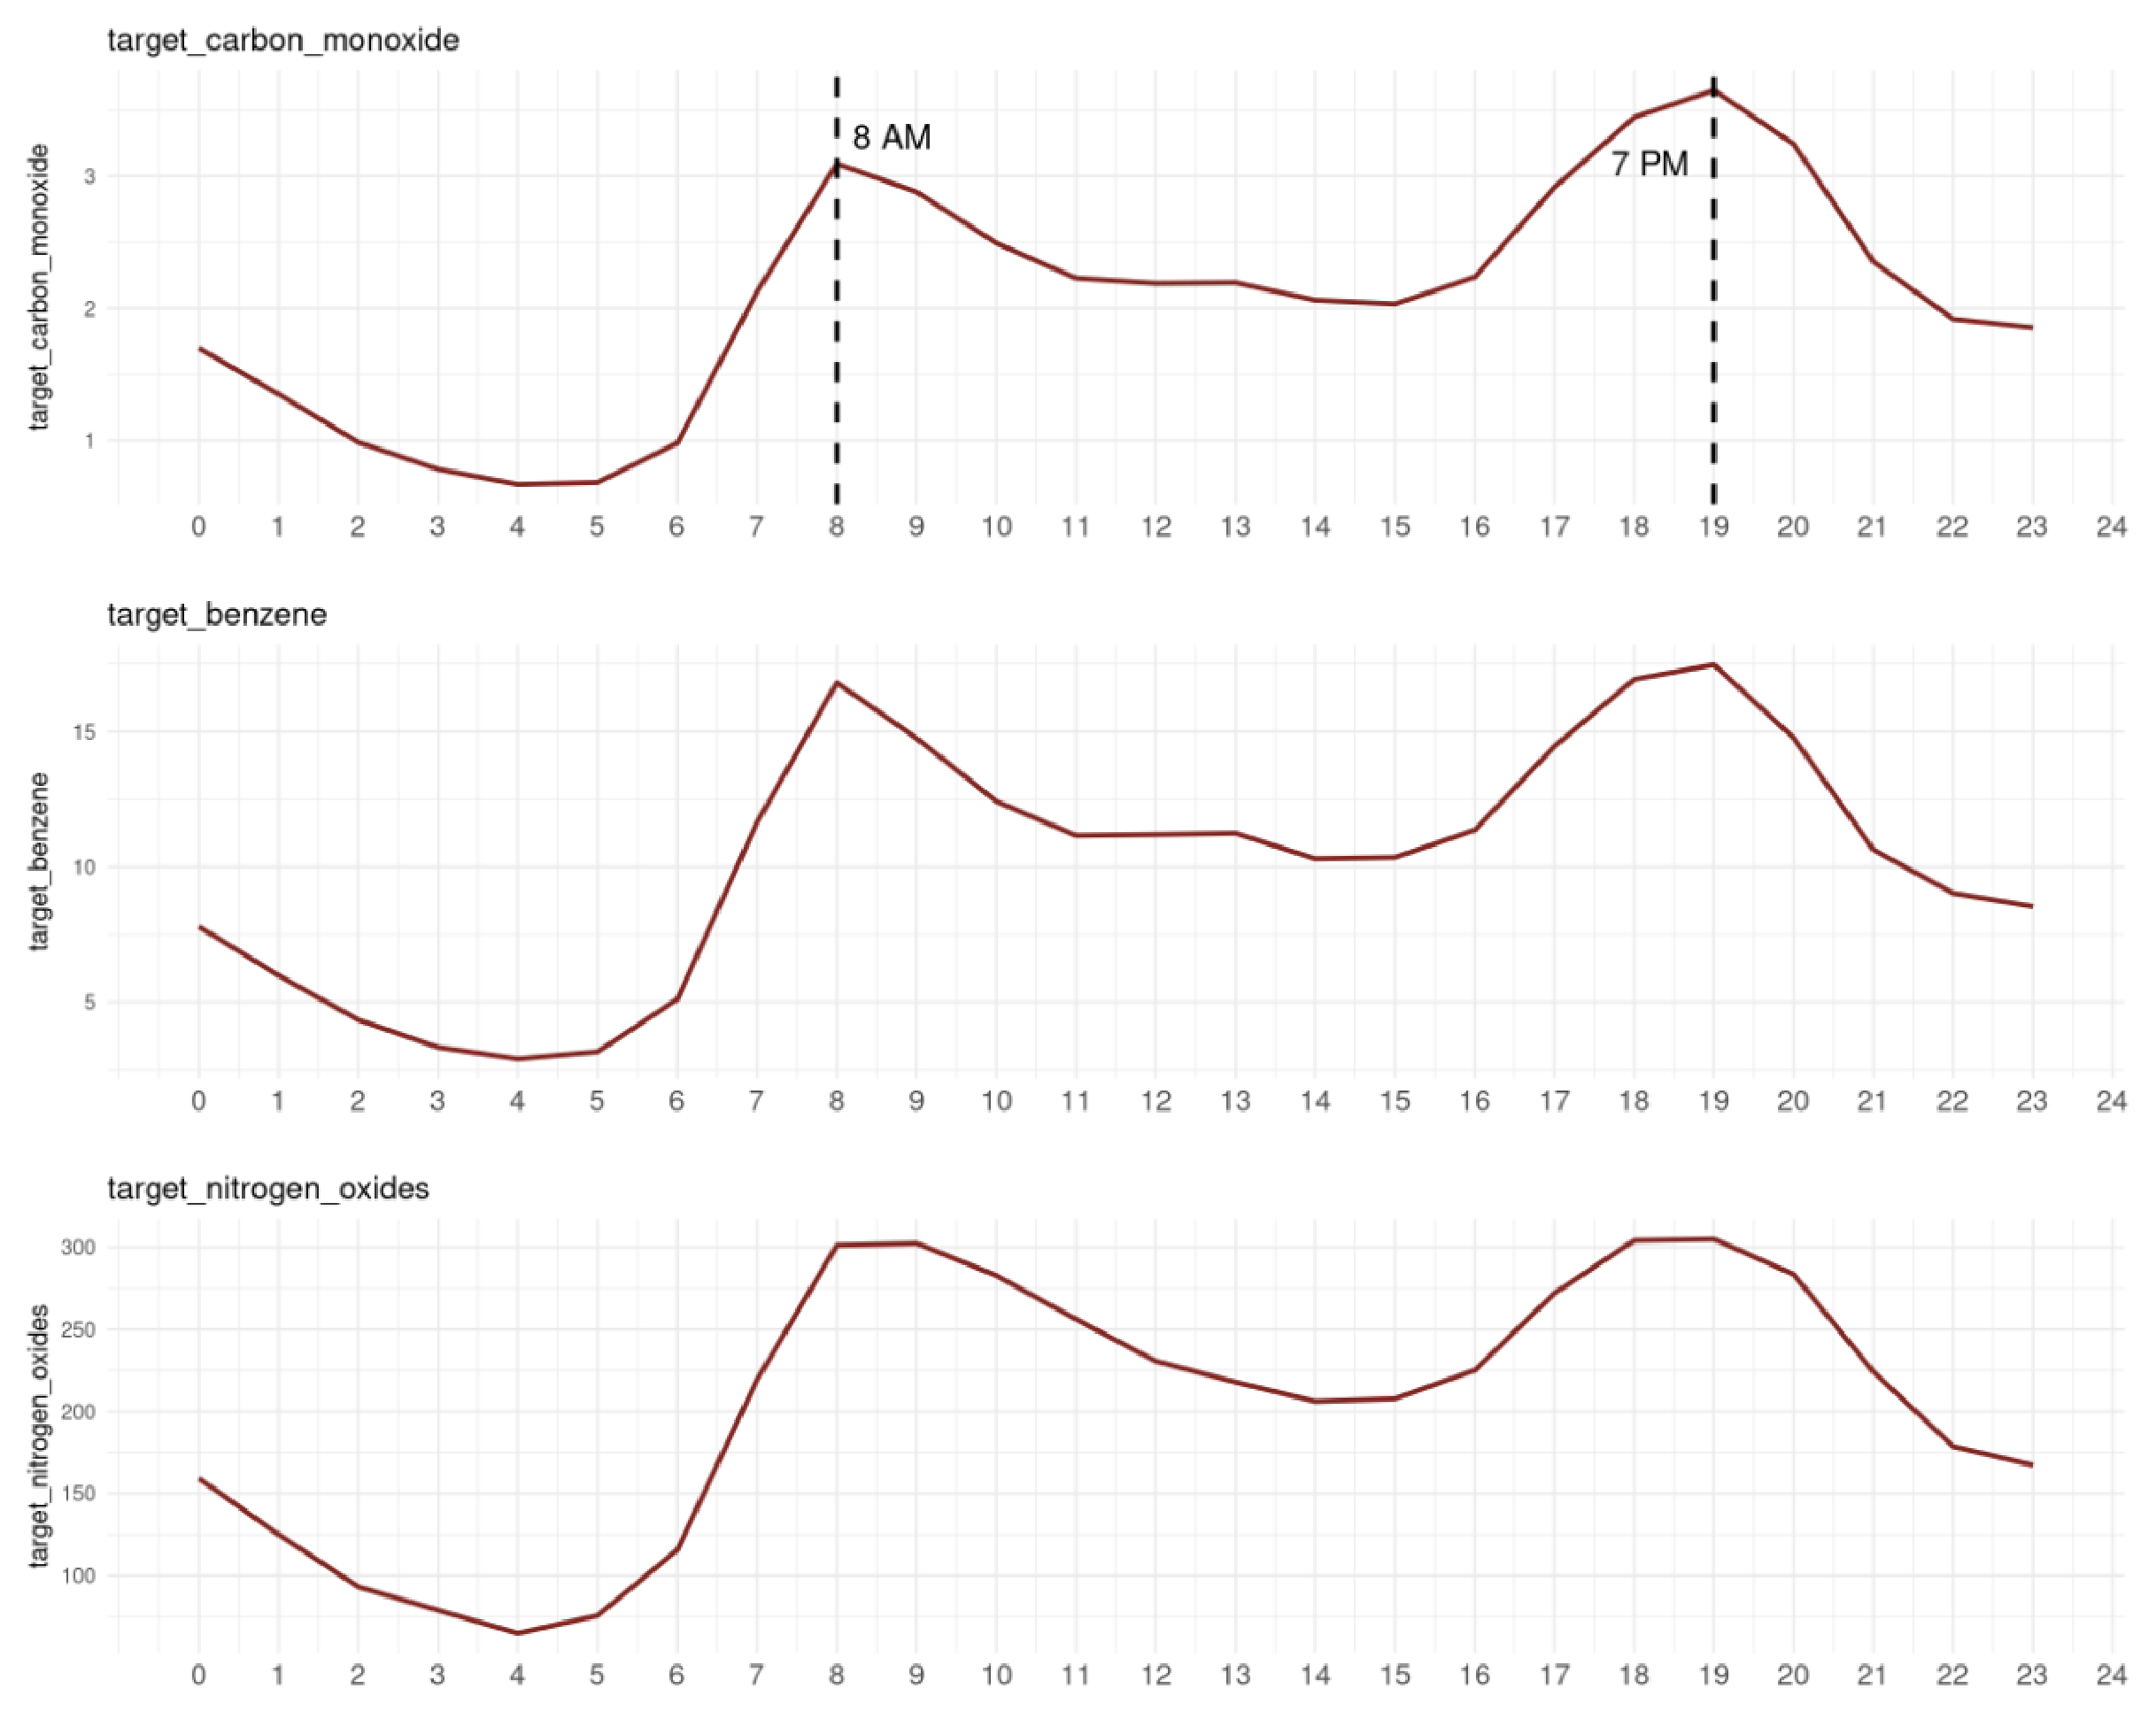
\includegraphics[scale=0.3]{figures//p5.eps}\\
	\caption{Target Daily Hourly Change}\label{fig:Target Daily Hourly Change}
\end{figure}
It can be seen from the figure3 that the level of each pollutant is the lowest at 5:00 a.m. every day, and then gradually rises to 8:00 a.m. to reach the first peak, and then gradually falls to 4:00 p.m., and then rises to 7:00 p.m. to reach the second peak, and then continues to decline, so it is necessary to take time as a feature of the model.




\section{Feature Engineering} \label{sec-method}
According to the analysis of training data, the following features are used for model training:
\begin{itemize}
	\item absolute-humidity
	\item deg-C
	\item relative-humidity
	\item sensor1-5
	\item month
	\item week
	\item is-weekend
	\item hour
\end{itemize}


\section{Model Training} \label{sec-experiment}
Data fitting using LGBMRegressor, the algorithm is easy to use. 
It only needs to put the set features and three prediction targets into the model for training, 
but there is no parameter optimization, which has a certain impact on the training results.



\section{Result} \label{sec-conclusions}
\begin{itemize}
	\item
	\smallskip
	Use RMSLE(Root Mean Squared Logarithmic Error) to evaluate the results.
	\begin{figure}[H]
		\centering
		\selectcolormodel{rgb}
		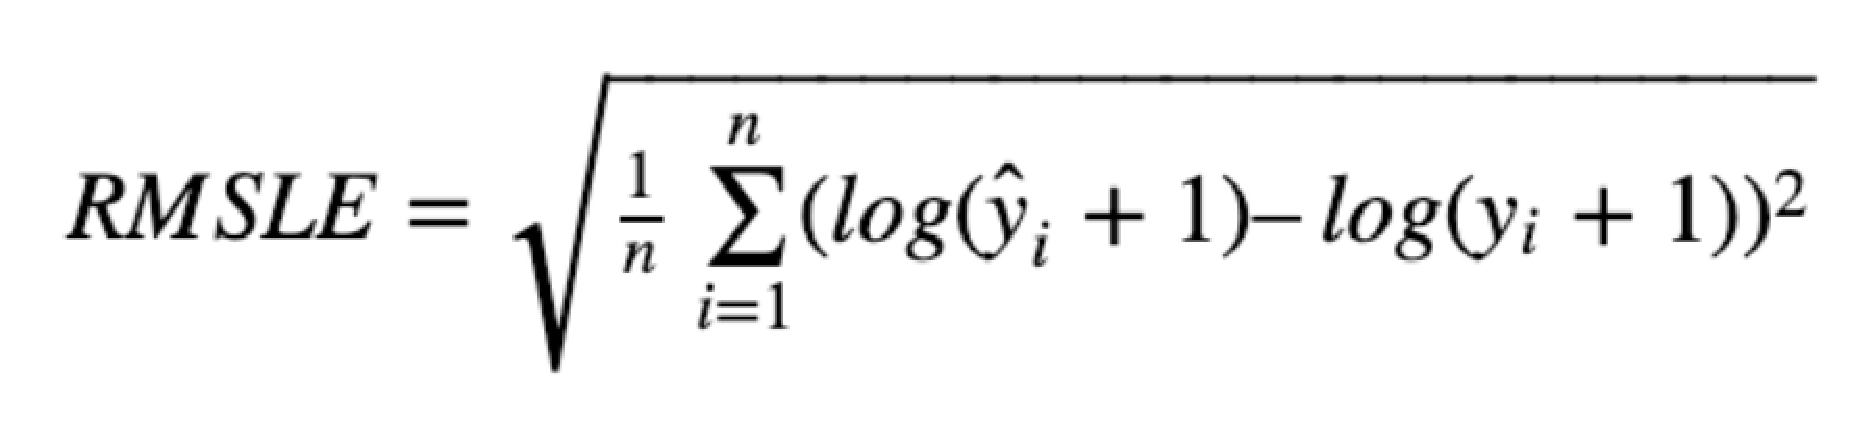
\includegraphics[scale=0.3]{figures//RMSLE.eps}\\
	\end{figure}
	
	
	\item
	\smallskip
	Private Score:0.33979
	
	\item
	\smallskip
	Public Score:0.387
	
\end{itemize}


